\chapter{Anforderungen}
\label{ch:requirements}
In diesem Kapitel werden die Anforderungen für den im vorherigen Kapitel aufgezeigten Anwendungsfall aufgestellt. Dazu werden zunächst einige Standards vorgestellt, wie Anforderungen klassifiziert und eingeordnet werden können. Diese Standards werden anschließend in einem Modell zusammengeführt und auf die konkreten Anforderungen angewandt. Abschließend werden alle typisierten Anforderungen auf \ac{DLT}-Relevanz geprüft und schrittweise reduziert, um letztlich diejenigen Anforderungen und deren Gruppierungen zu identifieren, die für die Umsetzung auf einer \ac{DLT}-basierten Lösung entscheidend sind.

%
% Section: Standards und Normen
%
\section{Standards und Normen}
\label{sec:requirements:standards}
In diesem Abschnitt werden

\subsection{BABOK}
\label{subsec:requirements:standards:BABOK}
\cite{BABOK}

\subsection{PMBOK}
\label{subsec:requirements:standards:PMBOK}
\cite{PMBOK}

\subsection{SWEBOK}
\label{subsec:requirements:standards:SWEBOK}
\cite{SWEBOK}

\subsection{SEBOK}
\label{subsec:requirements:standards:SEBOK}
\cite{SEBOK}

\subsection{ISO 29148}
\label{subsec:requirements:standards:ISO}
\cite{ISO29148}

\begin{figure}[htbp]
 \centering
 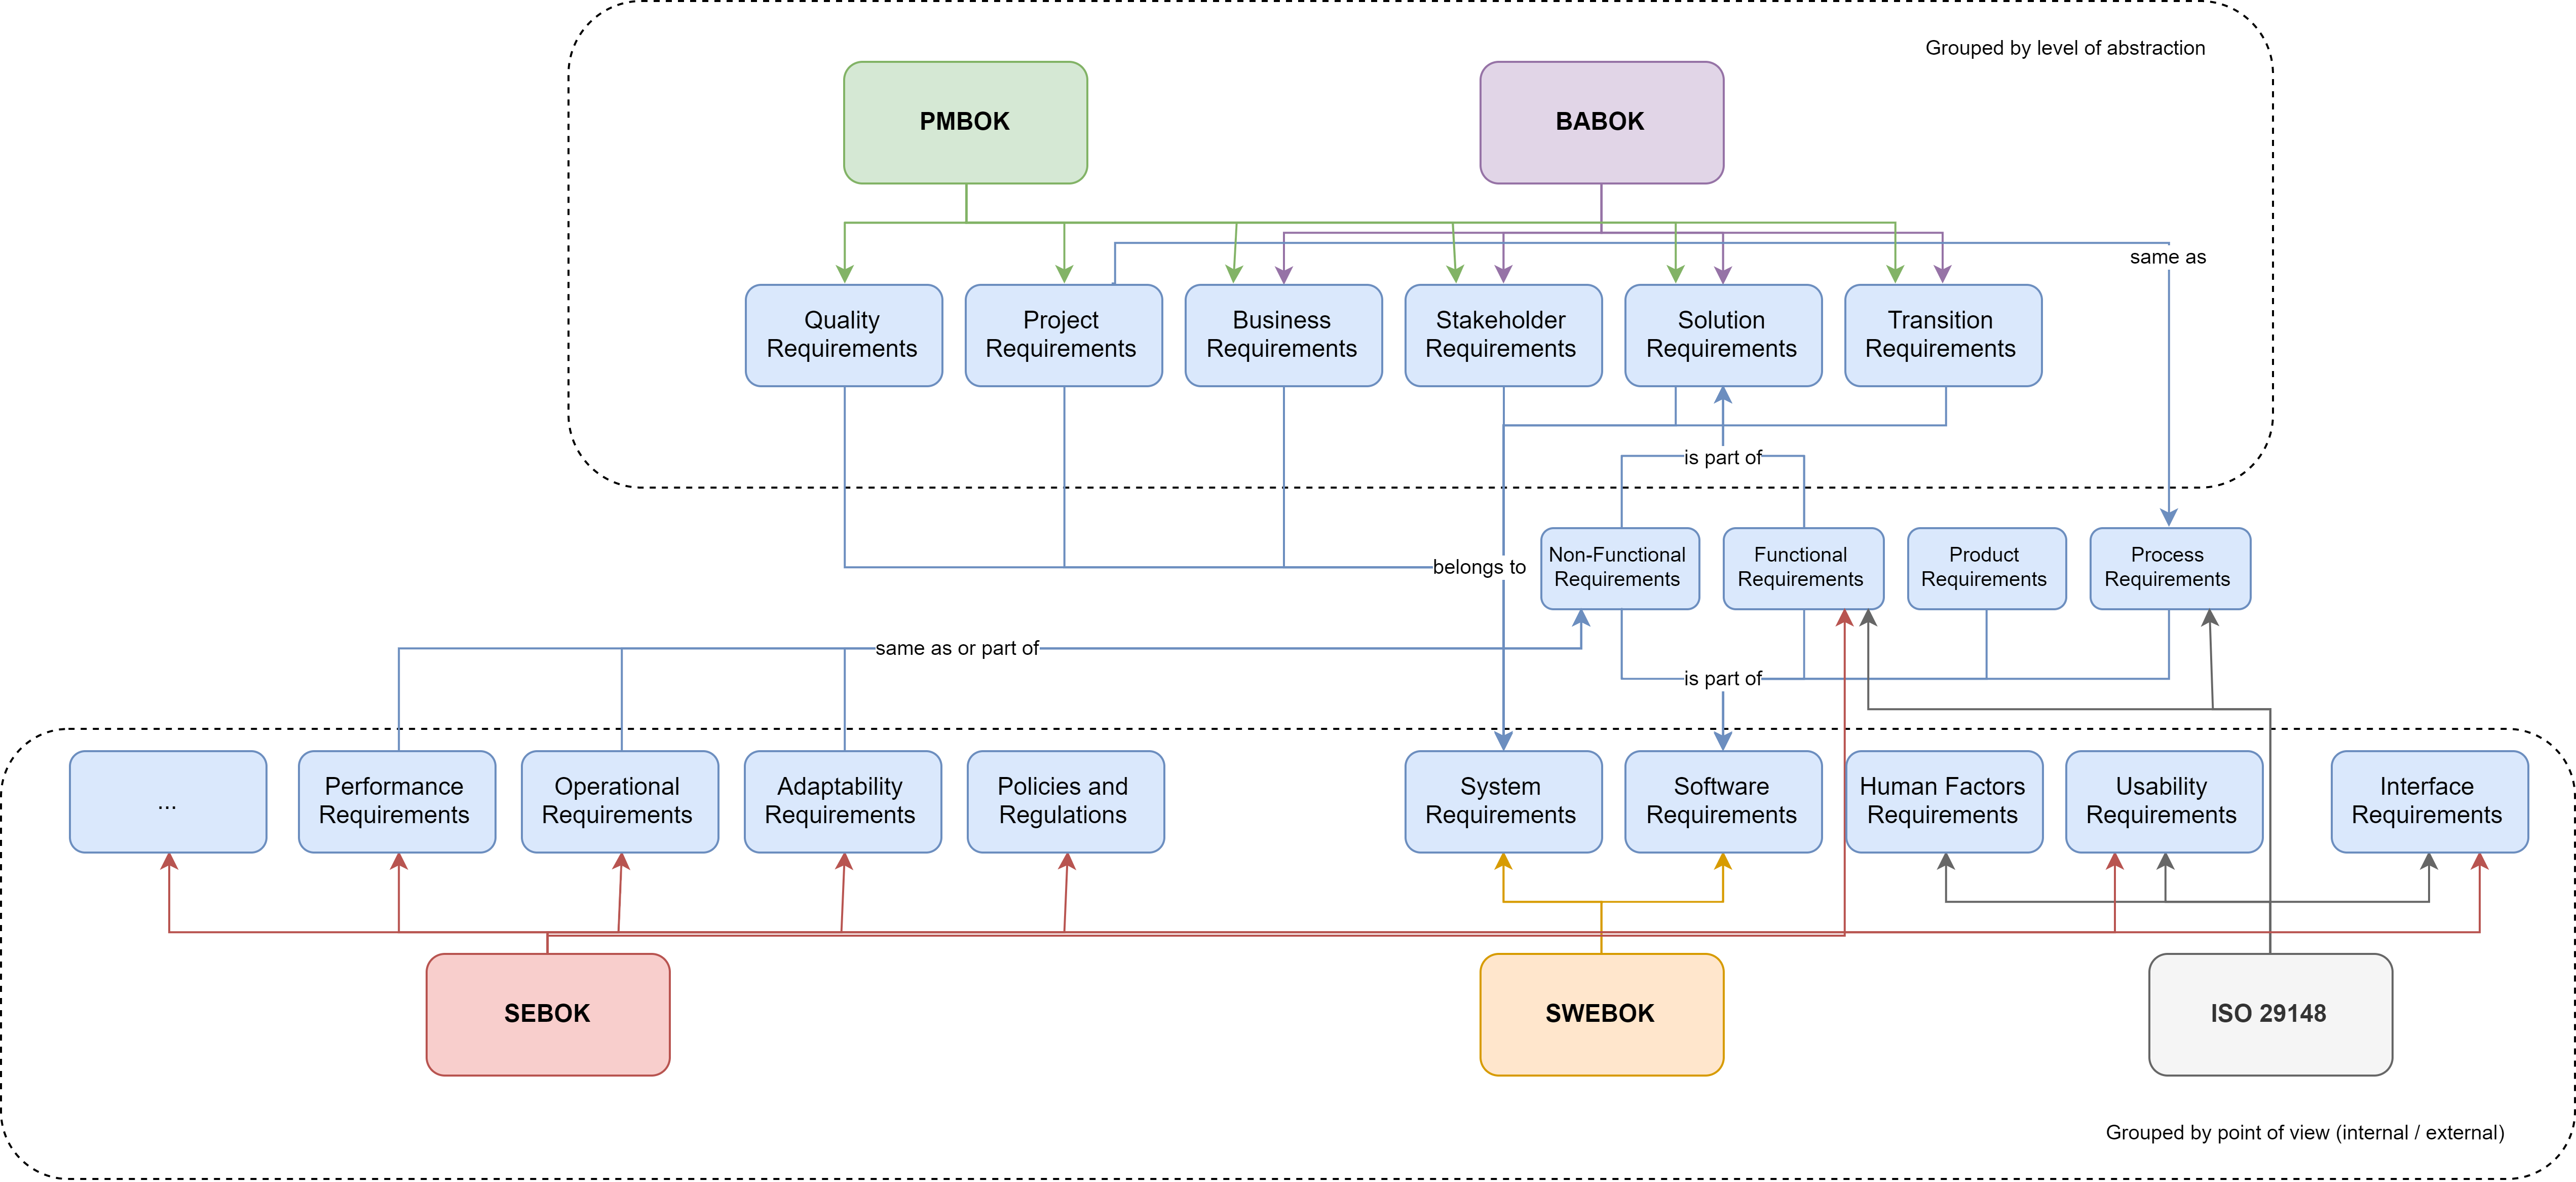
\includegraphics[width=1.0\textwidth]{gfx/Requirements.png}
 \caption{Einordnung der Begriffe und Zusammenhänge unterschiedlicher Normen und Standards}
 \label{fig:chapter05:requirements}
\end{figure}


\begin{figure}[htbp]
 \centering
 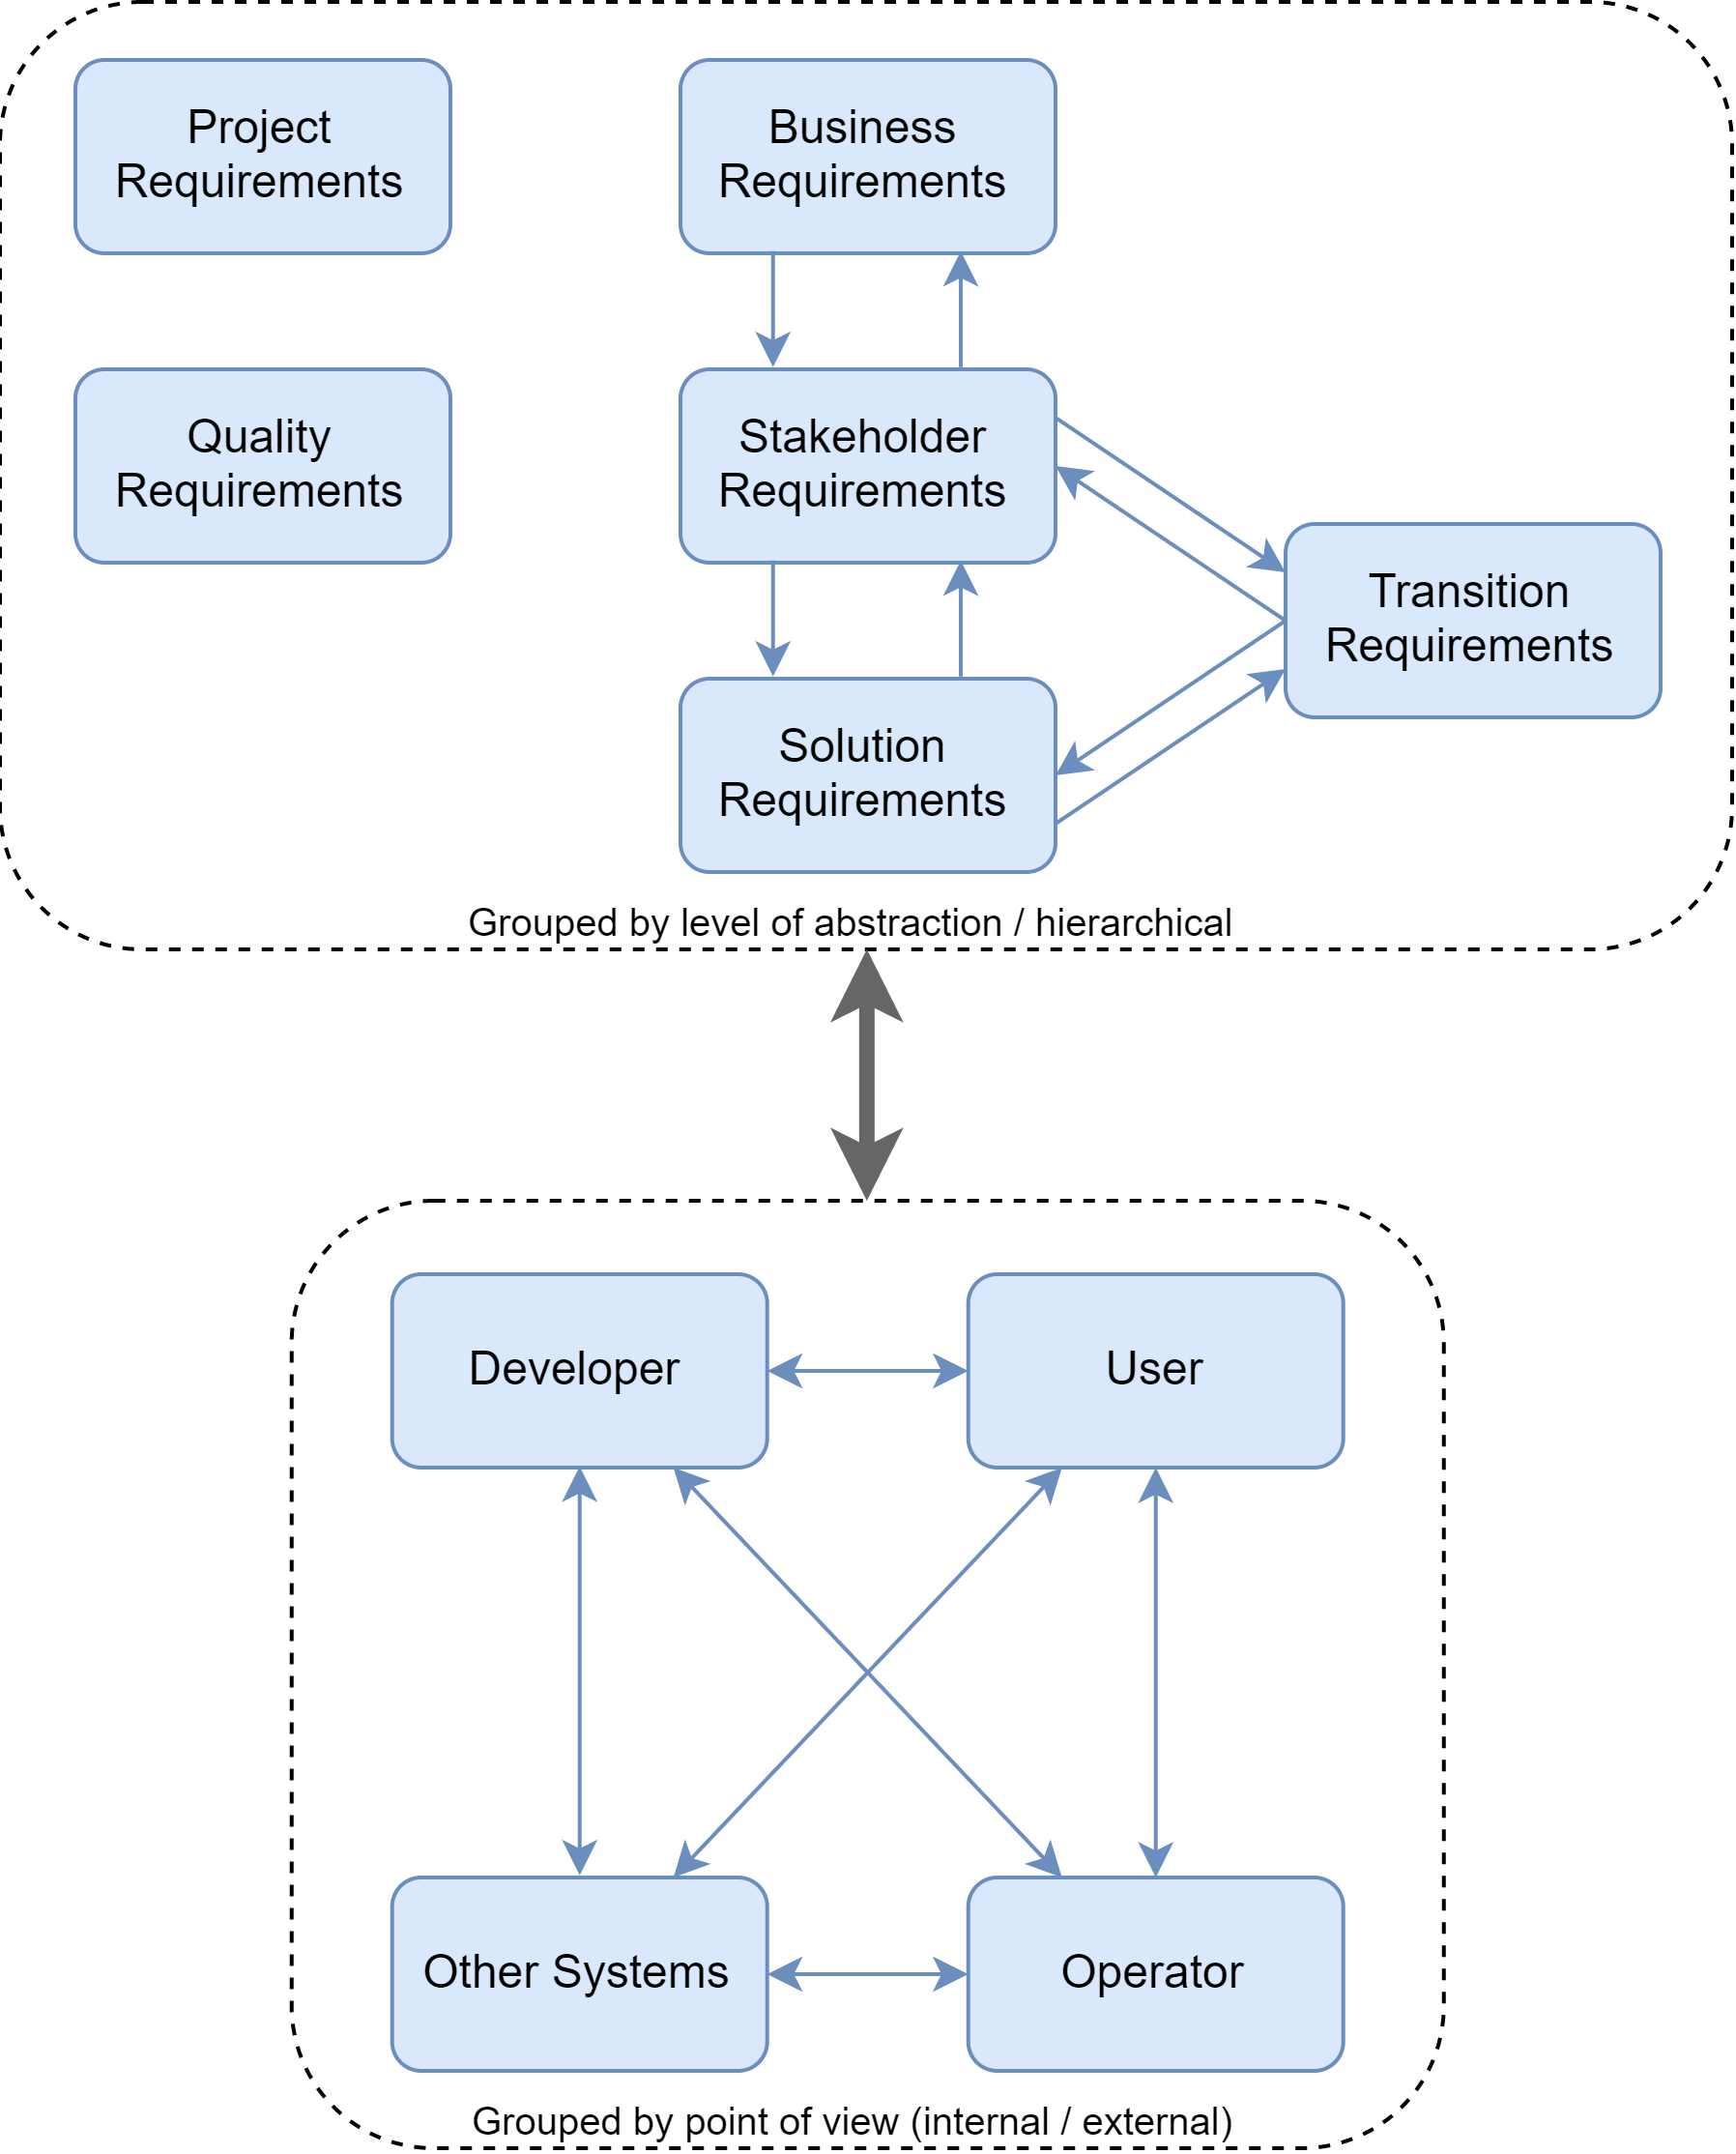
\includegraphics[width=1.0\textwidth]{gfx/Requirements_Grouping.png}
 \caption{}
 \label{fig:chapter05:requirements_grouping}
\end{figure}


\begin{figure}[htbp]
 \centering
 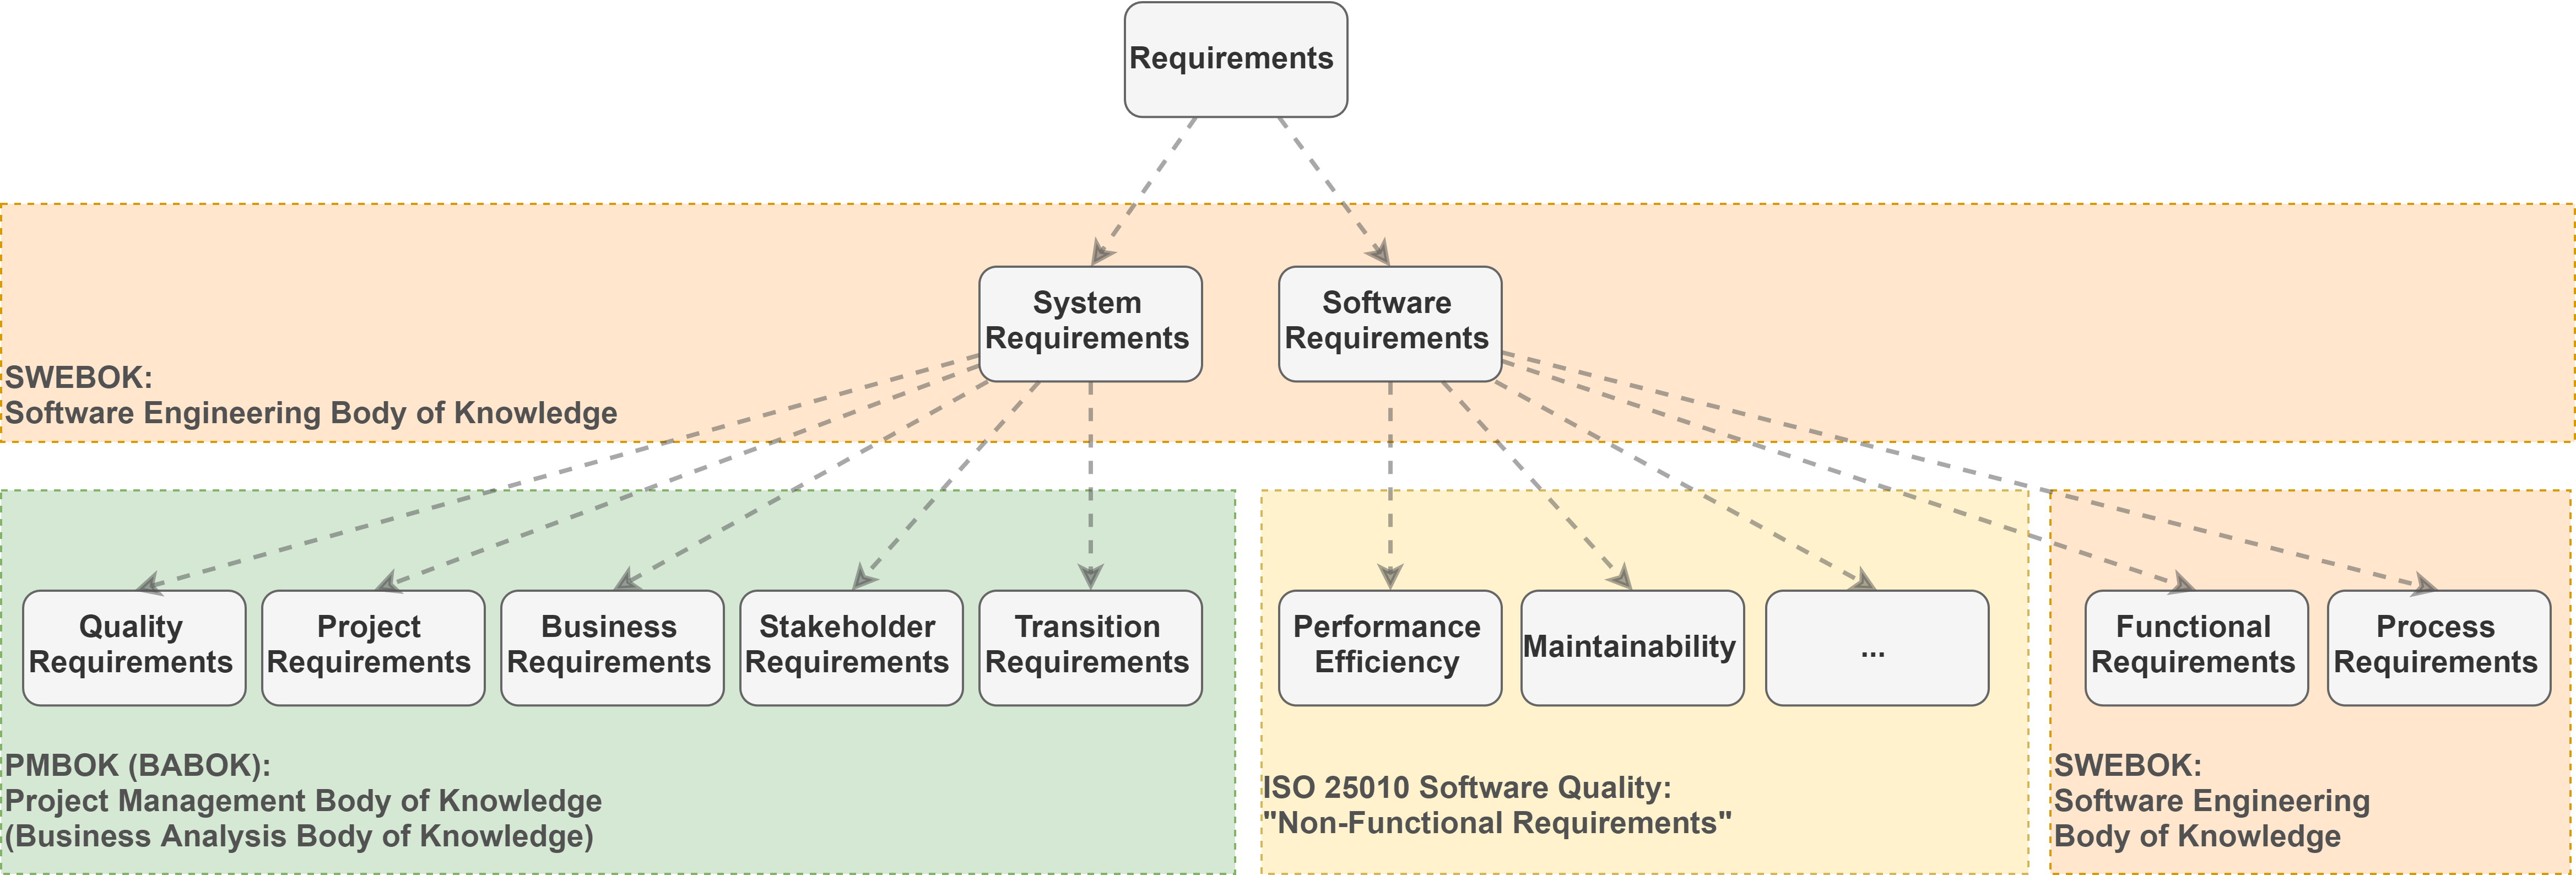
\includegraphics[width=1.0\textwidth]{gfx/Requirements_Hierarchy.png}
 \caption{}
 \label{fig:chapter05:requirements_hierarchy}
\end{figure}


%
% Section: Anforderungsanalyse
%
\section{Anforderungsanalyse}
\label{sec:requirements:analysis}
\lipsum[1-1]

%
% Section: Anforderungsklassifizierung
%
\section{Anforderungsklassifizierung}
\label{sec:requirements:classification}
\lipsum[1-1]

\subsection{Funktionale Anforderungen}
\label{subsec:requirements:classification:functional}
\lipsum[1-1]

\subsection{Nicht-Funktionale Anforderungen}
\label{subsec:requirements:classification:nonfunctional}
\lipsum[1-1]

\subsection{... Anforderungen}
\label{subsec:requirements:classification:other}
\lipsum[1-1]

%
% Section: Anforderungsevaluierung
%
\section{Anforderungsevaluierung}
\label{sec:requirements:evaluation}
\lipsum[1-1]
